\documentclass[]{myarticle}

\usepackage{mlbasemath}
\usepackage{mlcomplessita}

\makeatletter
\DeclareRobustCommand{\rvdots}{%
  \vbox{
    \baselineskip4\p@\lineskiplimit\z@
    \kern-\p@
    \hbox{.}\hbox{.}\hbox{.}
  }}
\makeatother

\usepackage{pgfplots}
\pgfplotsset{compat=1.5}
\usetikzlibrary{shapes,arrows,positioning,automata}

\usepackage[backend=bibtex]{biblatex}
\bibliography{multicore}

\author{Gabriele Atria \and Michele Laurenti}

\begin{document}

\title{Primo homework}
\maketitle

\section{Algoritmo ideale}

Trovare una password a forza bruta, conoscendone solo l'hash, equivale a cercare una stringa di lunghezza non determinata su un alfabeto.
Chiamiamo $\Sigma$ l'alfabeto su cui \`e costruita la stringa, e $\xi = \abs{\Sigma}$ il numero di caratteri nell'alfabeto.
La password che cerchiamo \`e una parola di $\Sigma^{\star}$ (l'insieme di tutte le parole costruite sull'alfabeto $\Sigma$).

L'idea algoritmica \`e la seguente: si enumerano tutte le stringhe in ordine quasi lessicografico (ordinandole prima per lunghezza, poi lessicograficamente), e si controlla se ciascuna di queste \`e la password cercata.
Se $n$ \`e la lunghezza della password, questo approccio permette di trovarla controllando non pi\`u di $\sum_{i = 1}^{n} \xi^i \simeq \xi^n$ stringhe.

Un'implementazione algoritmica \`e scegliere di creare un numero ``infinito'' di thread, assegnando a ciascuno una parola, e schedulare per primi i thread a cui \`e stata data una parola che viene prima nel nostro ordinamento.
Il programma temrina nel momento in cui un thread trova la stringa corrispondente alla password.
Il DAG di esecuzione di questo algoritmo sar\`a un albero con due livelli, e infiniti nodi sul secondo livello.

Con un solo processore a disposizione l'algoritmo visita i nodi da quello corrispondente alla parola pi\`u piccola a quello della password.
Possiamo quindi vedere il DAG con un solo processore come un cammino (figura \ref{fig:dag_seq}).
Assumendo che controllare se una stringa corrisponde alla password cercata abbia costo costante, il \emph{work} (tempo di esecuzione sequenziale) \`e $\bigo{\xi^n}$.

\begin{figure}[h]
	\centering
	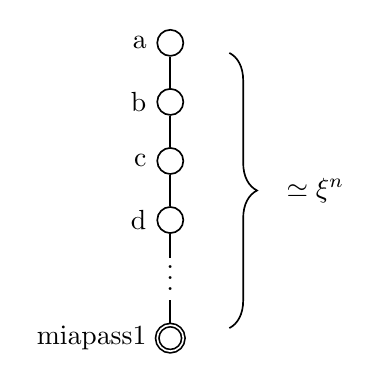
\begin{tikzpicture}[auto,semithick,node distance=.75cm]
		\node[circle,draw,label=left:a] (q0) {};
		\node[circle,draw,below of=q0,label=left:b] (q1) {};
		\node[circle,draw,below of=q1,label=left:c] (q2) {};
		\node[circle,draw,below of=q2,label=left:d] (q3) {};
		\node[below of=q3] (dots) {$\rvdots$};
		\node[circle,double,draw,below of=dots,label=left:miapass1] (qn) {};

		\node[right of=q0] (q0d) {};
		\node[right of=qn] (qnd) {};

		\draw (q0) -> (q1);
		\draw (q1) -> (q2);
		\draw (q2) -> (q3);
		\draw (q3) -> (dots);
		\draw (dots) -> (qn);
		\draw [decorate,decoration={brace,amplitude=10pt}]
		(q0d) -- (qnd) node [black,midway,xshift=0.6cm]
		{$\simeq \xi^{n}$};
	\end{tikzpicture}
	\caption{Il DAG di esecuzione dell'algoritmo sequenziale viene percorso come se fosse un cammino lungo circa $\xi^n$.}
	\label{fig:dag_seq}
\end{figure}

Con $p$ processori, invece, il DAG di esecuzione di questo algoritmo possiamo vederlo come un albero con $p$ figli, e ciascuno di questi figli \`e radice di un cammino lungo $\frac{\xi^n}{p}$ (figura \ref{fig:dag_par_p_proc}).

\begin{figure*}[th]
	\centering
	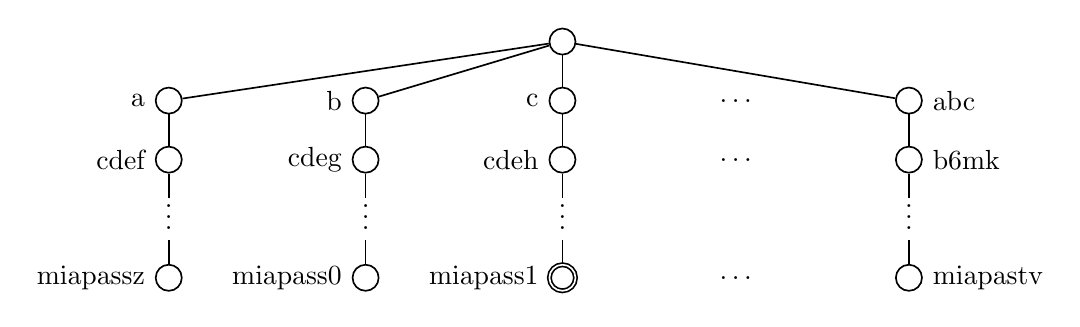
\begin{tikzpicture}[auto,semithick,node distance=.75cm]
		\node[circle,draw] (q0) {};
		\node[circle,draw,below of=q0,label=left:c] (q11) {};
		\node[circle,draw,node distance=2.5cm,left of=q11,label=left:b] (q21) {};
		\node[circle,draw,node distance=2.5cm,left of=q21,label=left:a] (q31) {};
		\node[right of=q11,node distance=2.2cm] (dots) {$\dots$};
		\node[circle,draw,node distance=2.2cm,right of=dots,label=right:abc] (q41) {};

		\node[circle,draw,below of=q31,label=left:cdef] (q32) {};
		\node[below of=q32] (3dots) {$\rvdots$};
		\node[circle,draw,below of=3dots,label=left:miapassz] (q3n) {};

		\node[circle,draw,below of=q21,label=left:cdeg] (q22) {};
		\node[below of=q22] (2dots) {$\rvdots$};
		\node[circle,draw,below of=2dots,label=left:miapass0] (q2n) {};

		\node[circle,draw,below of=q11,label=left:cdeh] (q12) {};
		\node[below of=q12] (1dots) {$\rvdots$};
		\node[circle,double,draw,below of=1dots,label=left:miapass1] (q1n) {};

		\node[circle,draw,below of=q41,label=right:b6mk] (q42) {};
		\node[below of=q42] (4dots) {$\rvdots$};
		\node[circle,draw,below of=4dots,label=right:miapastv] (q4n) {};

		\node[right of=q12,node distance=2.2cm] (dots1) {$\dots$};
		\node[right of=q1n,node distance=2.2cm] (dots2) {$\dots$};

		\draw (q0) -> (q11);
		\draw (q0) -> (q21);
		\draw (q0) -> (q31);
		\draw (q0) -> (q41);

		\draw (q11) -> (q12) -> (1dots) -> (q1n);
		\draw (q21) -> (q22) -> (2dots) -> (q2n);
		\draw (q31) -> (q32) -> (3dots) -> (q3n);
		\draw (q41) -> (q42) -> (4dots) -> (q4n);
	\end{tikzpicture}
	\caption{Il DAG di esecuzione dell'algoritmo parallelo \`e come un albero che ha come figli della radice $p$ cammini lunghi ciascuno $\frac{\xi^{n}}{p}$.}
	\label{fig:dag_par_p_proc}
\end{figure*}

Quindi il tempo di esecuzione con $p$ processori \`e $\bigo{\frac{\xi^n}{p}}$.
Quindi lo speedup \`e lineare con $p$.

Lo \emph{span}, ossia il tempo di esecuzione con un numero infinito di processori, \`e $\bigo{1}$: viene creato un numero infinito di thread, ciascuno su un processore, e ciascun thread controlla una sola parola.

\subsection{Ottimizzazione dell'algoritmo ideale}

La situazione illustrata \`e ideale e non prende in considerazione l'impossibilit\`a pratica di creare infiniti thread.
L'implementazione che proponiamo dell'algoritmo cerca per\`o di avvicinarsi alla situazione ideale, in cui la sincronizzazione non ha costi:
\begin{enumerate}
	\item \label{itm:opt_word_set} Ciascun thread non lavora su una singola parola alla volta, ma su un insieme di parole di cardinalit\`a fissata, per ridurre il numero di thread totali.
		\`E quindi necessario trovare una partizione di $\Sigma^{\star}$ le cui classi abbiano tutte la stessa cardinalit\`a, e che sia possibile ordinare linearmente in modo che la classe $A$  preceda la classe $B$  se e solo se tutte le parole di $A$ precedono in ordine quasi lessicografico tutte le parole di $B$.
		Se le due propriet\`a sono verificate gli elementi dell'insieme quoziente saranno insiemi di parole verificabili nello stesso tempo e ordinabili ``rispettando'' l'ordine quasi lessicografico delle parole.

		La partizione che proponiamo inserisce in una classe tutte le parole lunghe $k$ che hanno in comune i primi $j$ caratteri, dove $j < k$.
		La differenza $k - j$ deve essere un'invariante per tutte le classi di questa partizione.
	\item Non creiamo un numero infinito di thread, che \`e solo una utile astrazione mentale, ma ne creiamo un numero $m$ e cerchiamo per quali valori di $m$ si ottiene lo speedup maggiore.
		In questa implementazione deve esistere un metodo che atomicamente ritorna una diversa stringa su $\Sigma$ in ordine quasi lessicografico, o meglio una classe di stringhe come da punto \ref{itm:opt_word_set}.
		Ciascun thread chiama questo metodo e controlla le stringhe che riceve.
\end{enumerate}

\section{Implementazione}

\subsection{Piattaforma dei test}

I computer su cui abbiamo testato l'algoritmo sono:
\begin{itemize}
	\item Raspberry Pi 2 Model B, con CPU ``900 MHz quad-core ARM Cortex-A7'' secondo wikipedia \cite{wikipi}.
	\item MacBook Air (Early 2014), con CPU ``1.4 GHz (i5-4260U) dual-core Intel Core i5'' secondo wikipedia \cite{wikiair}.
\end{itemize}

Nei test condotti abbiamo fissato la lunghezza della password e generato password casuali di questa lunghezza, assieme all'ultima password in ordine quasi lessicografico di quella lunghezza.
Con lunghezza 4, il programma deve cercare $n$ password di lunghezza 4 e l'hash della password ``\code{9999}''.
Evitiamo quindi casi limite in cui le $n$ password generate sono tutte ``vicine'' e con un basso indice quasi lessicografico, costringendo il programma a provare (almeno) tutte le parole da ``\code{a}'' a ``\code{9999}''.

La lunghezza delle password \`e stata scelta da computer a computer, per arrivare a test della durata di qualche ora.

\subsection{Implementazione ingenua}

La prima implementazione che proponiamo ricalca grossomodo l'algoritmo ideale.
Rappresentiamo ogni parola con una \code{String}, e attraverso due generatori di stringhe (\code{AllStringGenerator}, globale e sincronizzato, e \code{StringGenerator}, locale a ciascun thread) forniamo ai thread creati un ``inizio'' di parola e lasciamo loro il compito di concatenare questo inizio con tutte le possibili combinazioni di $n$ lettere.

Le parole di lunghezza minore o uguale di $n$ (soglia che deve essere scelta opportunamente) vengono controllate in sequenziale all'inizio del programma.

Ciascun thread lavora su un insieme di parole e si sincronizza all'inizio del lavoro con la classe \code{Master} per ottenere l'insieme di password non ancora trovate.
Abbiamo scelto questa implementazione per evitare di dover mettere a disposizione dei thread un insieme di password sincronizzato (con lock di scrittura e di lettura), che avrebbe comportato l'acquisizione e il rilascio di un lock a ogni parola controllata.
Il draw-back di questa scelta \`e che i thread non termineranno il lavoro nel momento in cui l'ultima password viene trovata, ma se l'insieme di password su cui i thread lavorano \`e di dimensione ridotta l'attesa diviene trascurabile.

La struttura delle classi \`e rappresentata in figura \ref{fig:classi_progetto}.

\begin{figure*}[th]
	\centering
	\includegraphics[width=\textwidth]{homework1_classes.eps}
	\caption{Struttura delle classi del progetto.}
	\label{fig:classi_progetto}
\end{figure*}

\subsubsection{Risultati attesi}

\begin{itemize}
	\item Speedup lineare.
	\item Speedup massimo quando il numero di thread \`e uguale al numero dei processori.
	\item Buon load balancing.
\end{itemize}
I primi due risultati sono facilmente visibili.

\subsubsection{Risultati ottenuti}


% TODO illustrare i tempi di esecuzione

\begin{figure}[hp]
\resizebox{\columnwidth}{!}{
	\begin{tikzpicture}
		\begin{axis}[
			xtick=data,
			ymajorgrids,
			ymin=0.1,
			xlabel={\# thread},
			ylabel={tempo ($s$)},
		]
			\pgfplotstableread{plot.dat}{\risultatipi}
			\addplot[mark=o,red] table[x=threads,y=media] {\risultatipi};
			\pgfplotstablegetelem{0}{media}\of{\risultatipi};
			\pgfmathsetmacro{\yn}{\pgfplotsretval};
    		\addplot[domain=1:8,dashed,samples=400] (x,{\yn/x});
			\addplot[domain=1:8,dashed] {\yn/3};
			\node[] at (axis cs:2,\yn/3) {$\frac{1}{x}$};
  		\end{axis}
	\end{tikzpicture}
	}
	\caption{Tempo/thread su Raspberry Pi contro un insieme di parole di 4 lettere, con Oracle JVM.}
\end{figure}

\begin{figure}[hp]
\resizebox{\columnwidth}{!}{
	\begin{tikzpicture}
		\begin{axis}[
			xtick=data,
			ymajorgrids,
			ymin=0.1,
			xlabel={\# thread},
			ylabel={tempo ($s$)},
		]
			\pgfplotstableread{plot_openjdk.dat}{\risopenjdk}
			\addplot[mark=o,green] table[x=threads,y=media] {\risopenjdk};
			\pgfplotstablegetelem{0}{media}\of{\risopenjdk};
			\pgfmathsetmacro{\rpoyn}{\pgfplotsretval};
    		\addplot[domain=1:8,dashed,samples=400] (x,{\rpoyn/x});
			\addplot[domain=1:8,dashed] {\rpoyn/4};
			\node[] at (axis cs:2,\rpoyn/3) {$\frac{1}{x}$};
  		\end{axis}
	\end{tikzpicture}
	}
	\caption{Tempo/thread su Raspberry Pi contro un insieme di parole di 4 lettere, con OpenJDK.}
\end{figure}

\begin{figure}[hp]
\resizebox{\columnwidth}{!}{
	\begin{tikzpicture}
		\begin{axis}[
			xtick=data,
			ymajorgrids,
			ymin=0.1,
			xlabel={\# thread},
			ylabel={tempo ($s$)},
		]
			\pgfplotstableread{plot_2.dat}{\risultatipi}
			\addplot[mark=o,blue] table[x=threads,y=media] {\risultatipi};
			\pgfplotstablegetelem{0}{media}\of{\risultatipi};
			\pgfmathsetmacro{\yn}{\pgfplotsretval};
    		\addplot[domain=1:8,dashed,samples=400] (x,{\yn/x});
			\addplot[domain=1:8,dashed] {\yn/3};
			\node[] at (axis cs:2,\yn/3) {$\frac{1}{x}$};
  		\end{axis}
	\end{tikzpicture}
	}
	\caption{Tempo/thread su Raspberry Pi contro un insieme di parole di 5 lettere, con Oracle JVM.}
\end{figure}

\begin{figure}[hp]
\resizebox{\columnwidth}{!}{
	\begin{tikzpicture}
		\begin{axis}[
			xtick=data,
			domain=1:8,
			ymajorgrids,
			xlabel={\# thread},
			ylabel={speedup},
        ]
			\pgfplotstableread{plot.dat}{\risultatipi}
			\pgfplotstableread{plot_2.dat}{\risultatipibis}
			\pgfplotstableread{plot_openjdk.dat}{\risopenjdk}
			\addplot[mark=o,red] 
			 table[x=threads,y=speedup]  {\risultatipi};
			 \addlegendentry{Oracle JVM, 4 letters}
			\addplot[mark=o,blue] 
			 table[x=threads,y=speedup]  {\risultatipibis};
			 \addlegendentry{Oracle JVM, 5 letters}
			\addplot[mark=o,green]
			 table[x=threads,y=speedup]  {\risopenjdk};
			 \addlegendentry{Open JDK, 4 letters}
			\addplot[dashed,blue] {x};
			\addplot[dashed] {4};
			\node[above] at (axis cs:2,4) {\# processori};
		\end{axis}
	\end{tikzpicture}
	}
	\caption{Speedup/thread su Raspberry Pi.}
\end{figure}
% TODO illustrare i bottleneck, principalmente il garbage collector e l'uso di troppi oggetti immutabili

\subsection{Ottimizzazione del'implementazione}

Ogni thread, invece di creare ogni volta stringhe (tipi immutabili) che il garbage collector deve poi raccogliere, pu\`o mantenere un array di byte in cui inserisce di volta in volta la nuova parola.
MD5 prende in input un array di byte, e d\`a in output un array di byte, e guadagnamo non dovendo fare la conversione.
Conviene rappresentare anche gli hash in input come array di byte, e usare il metodo \code{Arrays.equals(byte[], byte[])} per i confronti.

% TODO illustrare i cambiamenti fatti

\subsubsection{Risultati ottenuti}

% TODO illustrare i tempi di esecuzione

\section{Conclusioni}

L'algoritmo non ha problemi di fiducia: nel momento in cui assegna un inseme di parole a un thread, assume che questo le controlli tutte.

Se eseguito su pi\`u computer l'algoritmo deve tenere traccia degli insiemi di parole che ha distribuito per assegnare a un nuovo \emph{worker} insiemi che restano ``orfani'' in caso di fallimenti.

\renewcommand{\refname}{Riferimenti}
\nocite{*}
\printbibliography

\end{document}

